\chapter{Empirical Characteristics of Returns}
\label{chap:1}

The modeling of asset returns has numerous applications, ranging from risk management to asset valuation over time. It is built upon a multi-theoretical foundation in time series analysis and financial theory, drawing insights from a wide range of disciplines. However, modeling asset returns remains an empirical craft, and practical relevance is demanded of these models. This should not come as a surprise, for financial markets are not mere theoretical abstractions; they are living, breathing systems that evolve and play a crucial role in the global economy.

\citeA{Campbell1997} give two main reasons for using returns instead of prices. First, for the average investor, the return of an asset provides a complete and scale-free summary of the investment opportunity. Second, for theoretical and empirical reasons that will become apparent, return series have attractive statistical properties.

We start by defining the daily continuously compounded or log return of an asset from the closing prices of the asset:
\[
R_{t+1}=\ln(S_{t+1})-\ln(S_{t})
\]
where $\ln(*)$ denotes the natural logarithm.

Most financial asset returns exhibit common empirical characteristics—what \citeA{Christoffersen2012} calls the stylized facts of asset returns and what \citeA{Tsay2010} refers to as the empirical properties of returns. \textbf{These empirical characteristics serve as guidelines for what models should capture and replicate}. To illustrate each of these characteristics, we will use daily log returns of the S\&P 500 (Yahoo Finance ticker: \texttt{\textasciicircum{}GSPC}) from January 1, 2014, to December 31, 2024, with closing prices retrieved through the Yahoo Finance API.


Daily log returns exhibit very little autocorrelation. Formally, we can write
\[
\text{Corr}(R_{t+1},R_{t+1-\tau})\approx0 \quad \text{for } \tau = 1,2,3,\ldots \quad. 
\]
This implies that past returns possess little to no predictive power for future returns. Figure~\ref{1.1} displays the autocorrelation function (ACF) of daily S\&P 500 log returns for lags 1 through 100. For lag $\tau$, the ACF is defined as $\rho_\tau = \text{Corr}(R_{t+1},R_{t+1-\tau}).$ For example, at the first lag—that is, the correlation between today’s return and the previous day’s return—the estimated autocorrelation is $\rho_1 = -0.13$.

The dotted lines represent the 95\% confidence interval within which it is statistically reasonable to state that $\rho_\tau = 0$ (under a specific set of assumptions). In the time-series literature, these are commonly referred to as Bartlett’s confidence bands (see, for example, \citeA{Tsay2010}), and are given by $\pm 1.96/\sqrt{T}$. Although there are a few lags for which the estimated autocorrelation falls outside these bands, the overall magnitude of the autocorrelations is small. Given both their low magnitude and the daily frequency of the data, the models developed below assume that the conditional mean of returns is approximately constant, that is, that there is no meaningful linear dependence in returns.
\begin{figure}[H]
    \centering
    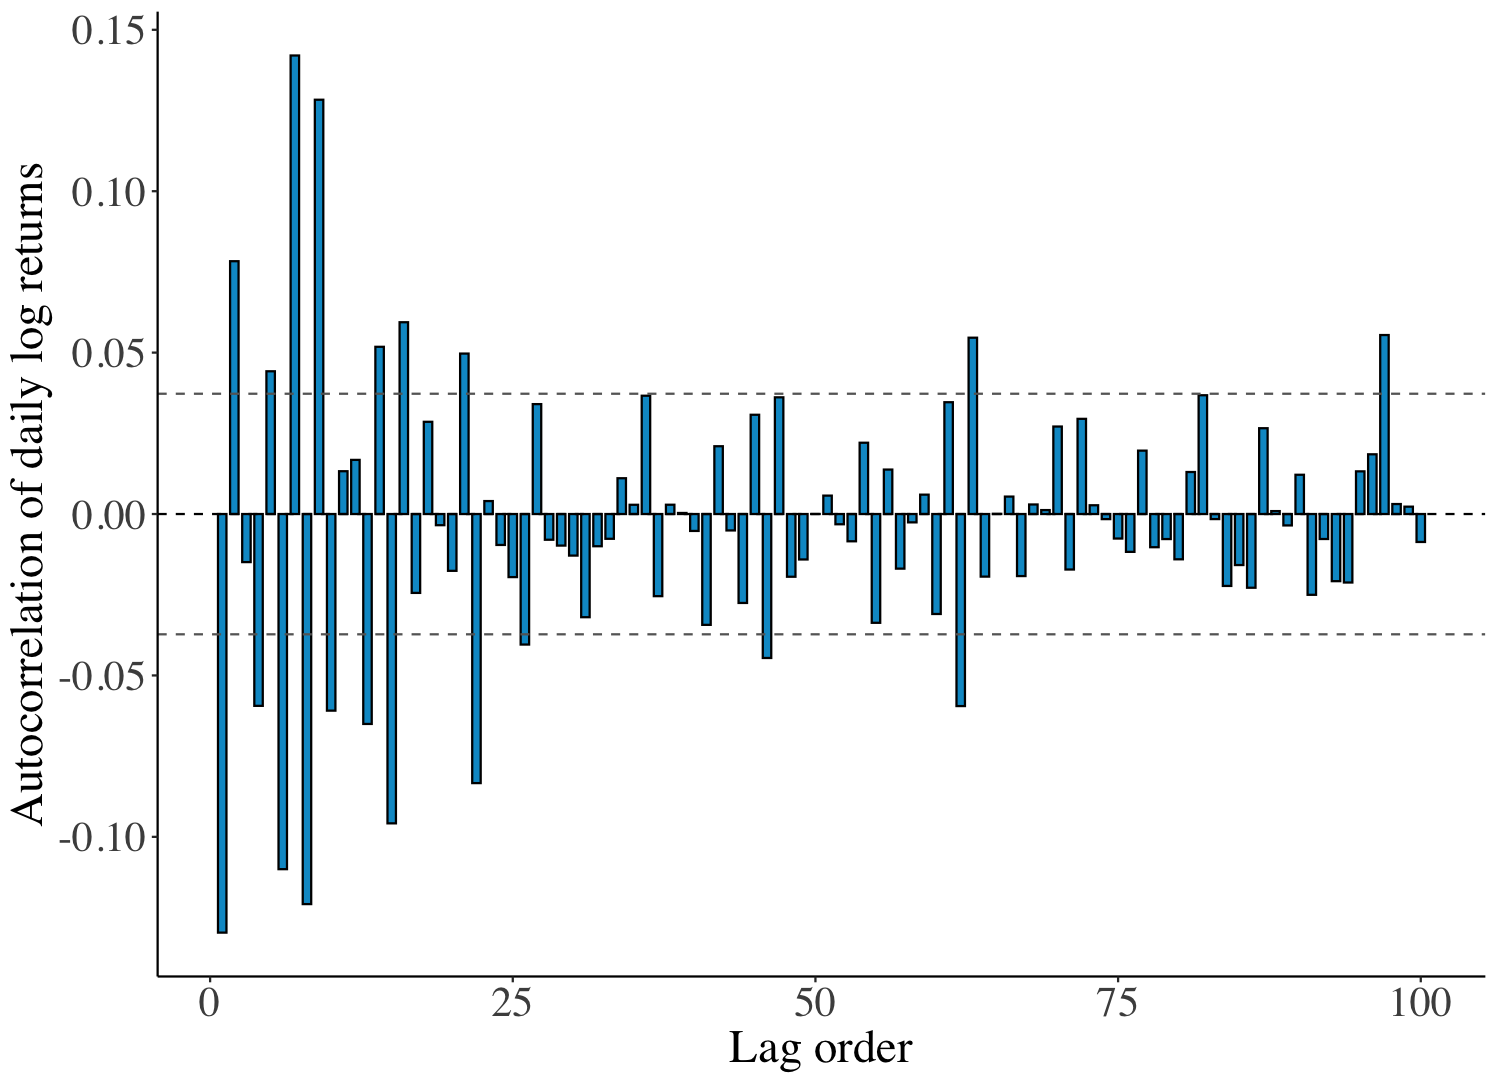
\includegraphics[scale=0.18]{../../plots/1.1.png}
    \caption{Autocorrelation of daily S\&P 500 log returns from January 1, 2014, to December 31, 2024.}
    \label{1.1}
\end{figure}

The unconditional distribution of daily returns departs from normality. Figure~\ref{1.2} shows a histogram of S\&P 500 daily log returns together with a normal density fitted by maximum likelihood. Several features stand out. First, the empirical distribution is more peaked around zero (i.e., leptokurtic). Second, it exhibits heavier tails than the normal, implying a higher probability of extreme outcomes. Third, the distribution is asymmetric: in this sample it displays left-skewness (negative skewness), with a longer left tail than the right. Accurately modeling tail behavior is crucial for risk management, as emphasized by \citeA{Christoffersen2012}.

\begin{figure}[H]
    \centering
    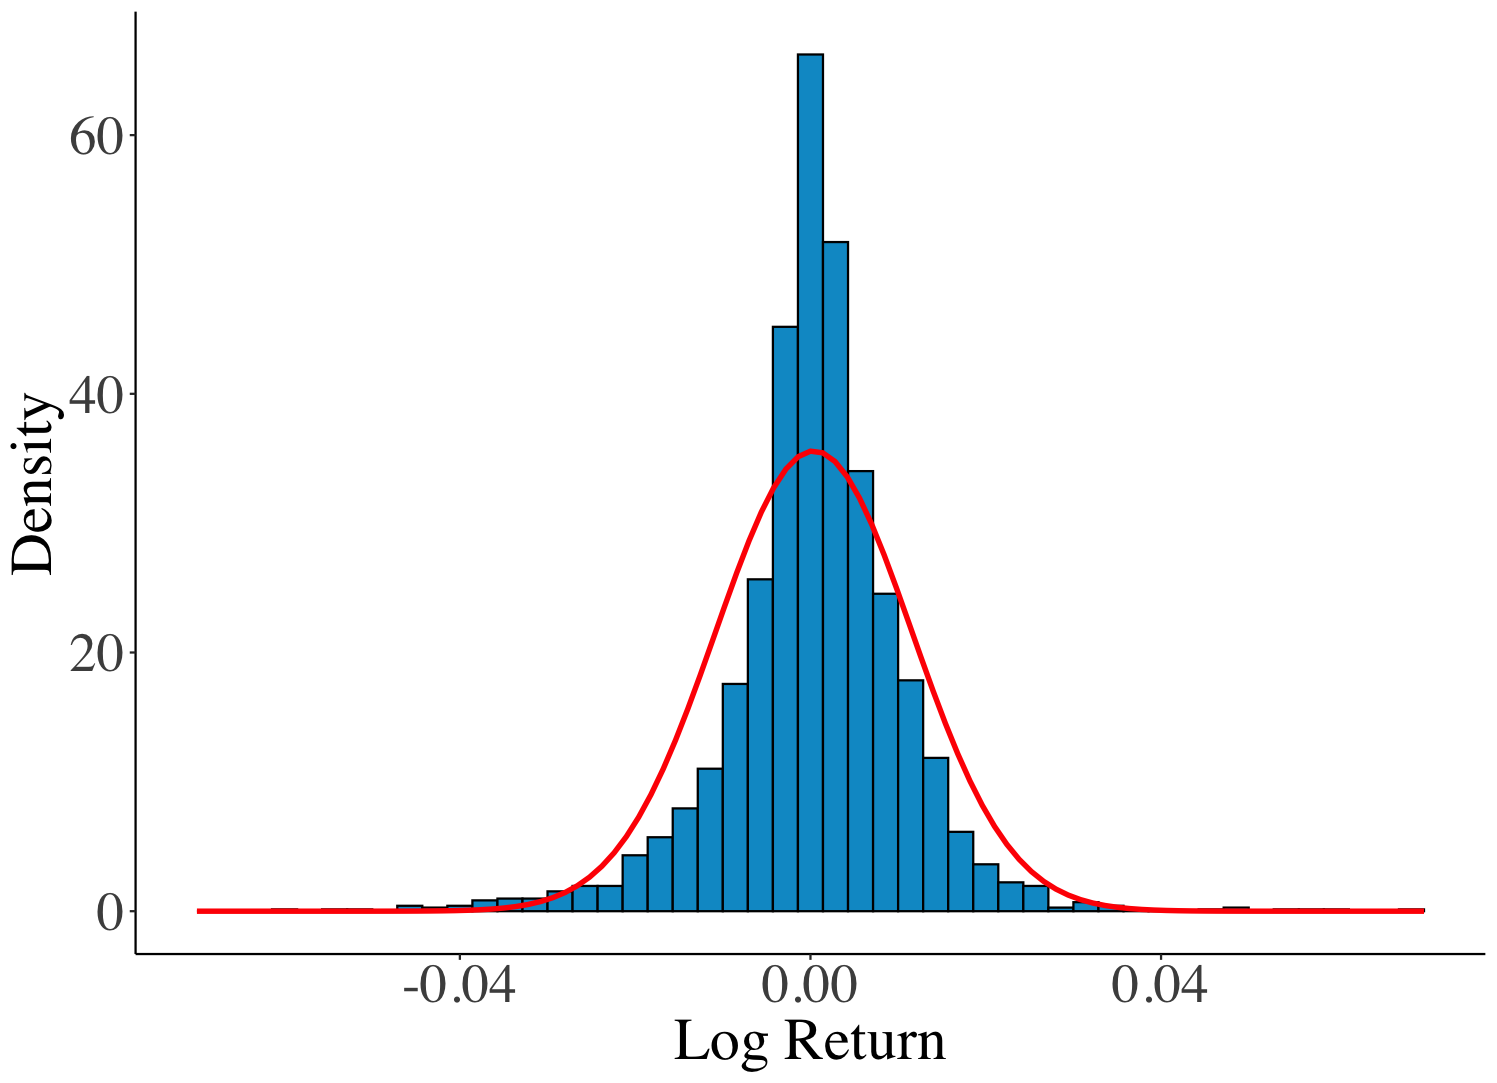
\includegraphics[scale=0.18]{../../plots/1.2.png} % Replace 
    \caption{Histogram of daily S\&P 500 log returns and the normal distribution January 1, 2014 - December 31, 2024. Skewness : -0.8088, Kurtosis : 19.0445   }
    \label{1.2}
\end{figure}

The stock market experiences sharp declines in stock prices and index values, but not equally large upward movements. Consequently, the return distribution exhibits negative skewness.

The standard deviation of returns is considerably larger than the mean at short horizons, such as daily. Statistically, it is reasonable not to reject a zero mean return. Our S\&P 500 data exhibit a daily mean return of 0.0380\% and a daily standard deviation of 1.1211\%.

\pagebreak

Volatility measures, such as squared returns\footnote{Squared returns are commonly used as measures of volatility because, under many return specifications (like the one we discuss below),
$\mathbb{E}[R_t^2 \mid R_{t-1}, R_{t-2}, \ldots] = \sigma_t^2$.
For this reason, the time series of squared returns, $\{R_t^2\}$, becomes relevant for studying volatility dynamics. As noted by \citeA{Christoffersen2012}, squared returns provide an unbiased, though noisy, proxy for conditional variance.}, exhibit positive correlation with their past values, reflecting the tendency of high-volatility events to cluster over time. This effect is most pronounced at short horizons, such as daily returns. Formally, we can write
\[
\text{Corr}(R^2_{t+1},R^2_{t+1-\tau}) > 0 \quad \text{for small } \tau. 
\]
Figure~\ref{1.3} shows the autocorrelation in squared returns for the S\&P 500 data. Models that account for this dependence will be introduced in the next section.

\begin{figure}[H]
    \centering
    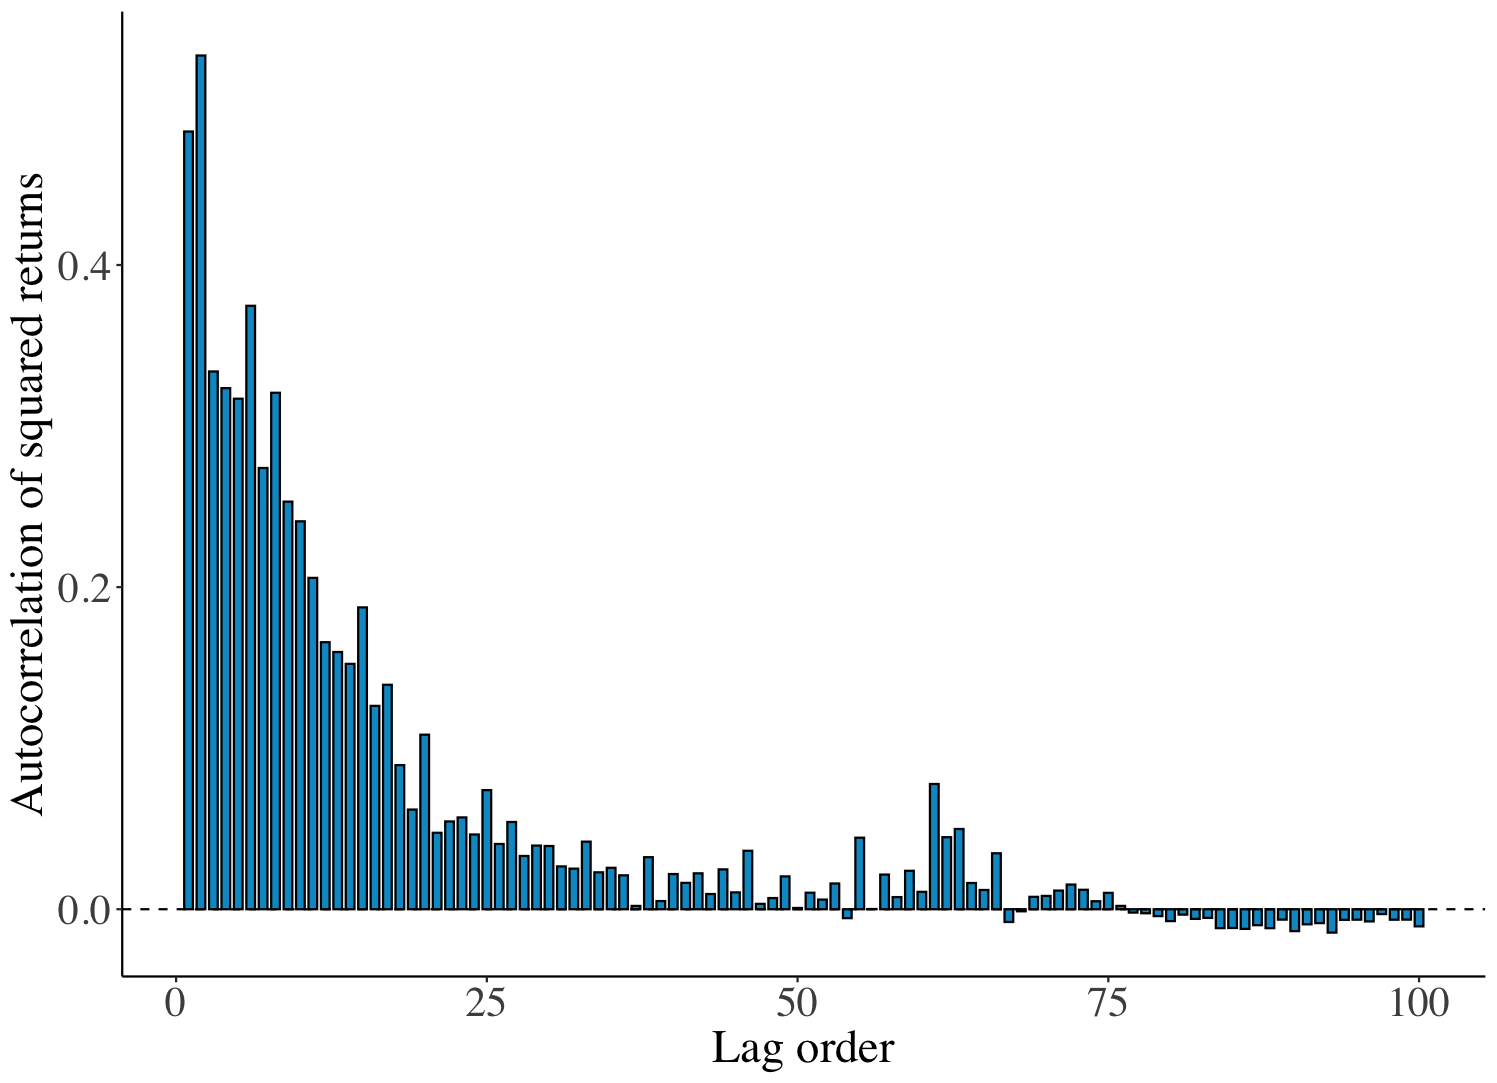
\includegraphics[scale=0.18]{../../plots/1.3.png} % Replace 
    \caption{Autocorrelation of squared daily S\&P 500 log returns from January 1, 2014, to December 31, 2024.}
    \label{1.3}
\end{figure}

For equities and equity indices, asset volatility is negatively correlated with returns. A negative return increases the (conditional) variance more than a positive return of the same magnitude. This phenomenon is known as the leverage effect, arising from the fact that a decrease in a stock’s price increases the firm’s leverage—assuming its debt remains constant—thereby making it riskier.

The correlation among assets appears to vary over time. Notably, it tends to increase in magnitude during highly volatile bear markets and spikes dramatically during market crashes. Figure~\ref{1.4} displays the rolling covariance between S\&P 500 returns and the returns on a 10-year Treasury note index (Bloomberg ticker: \texttt{SPBDU1BT Index}, retrieved via the Bloomberg Terminal), calculated using a 25-day rolling window. A sharp increase in covariance is evident during the early phase of the 2020 pandemic.

\begin{figure}[H]
    \centering
    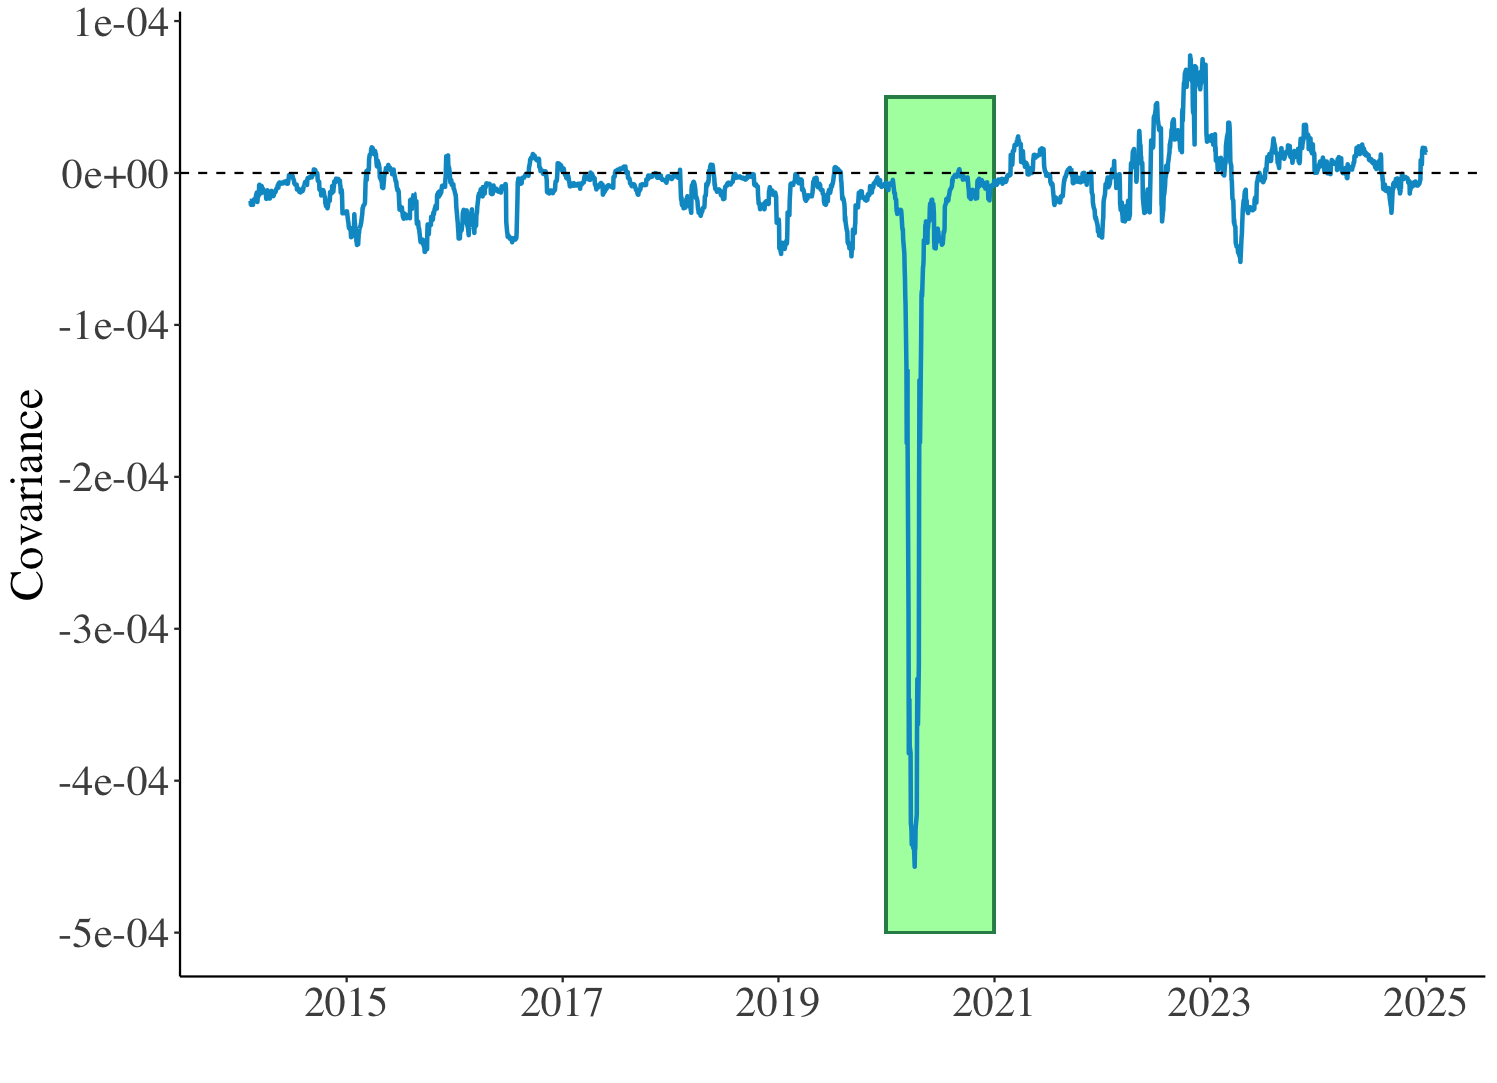
\includegraphics[scale=0.175]{../../plots/1.4.png} % Replace 
    \caption{Rolling covariance between S\&P 500 and 10-year treasury note index.}
    \label{1.4}
\end{figure}

Lastly, even after standardizing returns by time-varying volatility, they continue to exhibit heavier tails than the normal distribution. However, the tails are lighter than those in the unconditional return distribution. This provides evidence of conditional non-normality.

\citeA{Cont2001} provides a detailed discussion of the empirical characteristics of returns presented here, along with additional ones, and examines various statistical challenges that arise in the analysis of financial time series.

Considering the empirical behavior of returns, the model for individual asset returns is
\begin{equation}
R_{t+1}=\mu_{t+1} +\sigma_{t+1}z_{t+1} \quad \text{where } z_{t+1} \sim \text{i.i.d. } D(0,1).
\label{eq:1.1}
\end{equation}
The random variable $z_{t+1}$ represents the innovation term or shock, which we assume to be identically and independently distributed (i.i.d.) with zero mean and unit variance. We assume that the conditional mean of returns, $\mu_{t+1}$, is zero — a reasonable assumption based on the empirical behavior of daily returns discussed earlier. For longer horizons a model for the mean can be necessary\footnote{Readers interested in modeling the conditional mean, $\mu_{t+1}$, are referred to \citeA{Tsay2010} Chapters 2 and 4, and the references therein. \citeA{Tsay2010} provides an exhaustive review of linear and nonlinear models for the conditional mean in financial time series.}, here we focus on modeling daily returns. 

The specification for daily returns is then given by
\begin{equation}
    R_{t+1}=\sigma_{t+1}z_{t+1} \quad \text{where } z_{t+1} \sim \text{i.i.d. } D(0,1).
    \label{eq:1.2}
\end{equation}

\newpage
The univariate and multivariate return models developed in the subsequent chapters are designed to capture and replicate the empirical properties documented in this section. The next section models the conditional volatility, $\sigma_{t+1}$, and the following section models the standardized innovation, $z_{t+1}$.
